\documentclass{article}

\usepackage[utf8]{inputenc}
\usepackage{parskip}
\usepackage{graphicx}
\usepackage{epstopdf}
\usepackage{wrapfig}
\usepackage{mwe}
\usepackage{libertine}
\usepackage{inconsolata}
\usepackage{hyperref}

\newcommand\theversion{1.1.0-git}
\newcommand\thegame{One Man's Trash}

\hypersetup{
  hidelinks,
  pdftitle={\thegame{} v\theversion}
}

\setcounter{secnumdepth}{4}
\renewcommand{\sectionautorefname}{§}
\renewcommand{\subsectionautorefname}{§}
\renewcommand{\subsubsectionautorefname}{§}
\renewcommand{\paragraphautorefname}{¶}

\newcommand\copyrightfooter{
  \medskip
  \hrule

  {
    \small
    \includegraphics[scale=0.5]{cc-by.eps}\\
    This work is licensed under the Creative Commons Attribution 4.0
    International License. To view a copy of this license, visit
    \url{http://creativecommons.org/licenses/by/4.0/} or send a letter to Creative Commons, PO Box 1866, Mountain View, CA 94042, USA.
  }
}

\begin{document}
\title{\thegame{}\\ \large A card game, v\theversion}
\author{Johann Tutor}
\date{\today}
\maketitle

\tableofcontents

\newpage

\section{Requirements}
\label{sec:requirements}

\thegame{} requires 2 -- 6 players and a standard deck of cards (with 2 Jokers if available).

If Jokers are available, then these Jokers are considered the ``Trash Collectors''.

If Jokers are not available, remove two Aces.
The two remaining Aces are considered the Trash Collectors.

\section{Setup}
\label{sec:setup}

\begin{enumerate}
  \item Determine a player order.
  \item Shuffle the deck.
  \item Deal 3 cards to each player. The players may look at their dealt hands.
  \item Deal 3 cards face-up on the table to form three Trash Piles.
  \item Put the remaining cards face-down to form the Draw Pile.
\end{enumerate}

\section{Rules}
\label{sec:rules}

The aim of the game is to empty your hand by trashing a four-of-a-kind on to a Trash Pile.

\subsection{Gameplay}
\label{sec:gameplay}

Play proceeds in turns. On your turn, you must perform one of five actions: pick up from the Draw Pile, trash a card, collect the trash, litter, or swap a card.

If you run out of cards in your hand and you did not meet the win condition (\autoref{sec:winning}), you lose and are out of the game.

In addition, on your turn or between turns, you may inspect the Trash Piles (taking care not to disturb the order of the cards) or ask any player about the number of cards in their hand.

\newpage
\subsubsection{Pick Up From the Draw Pile}
\label{sec:draw}

On your turn, you may choose to draw from the Draw Pile to add a card to your hand.

\paragraph{} \label{par:drawnormal}
Draw one card from the Draw Pile and add it to your hand.

\paragraph{} \label{par:drawempty}
You may not pick up from the Draw Pile if the Draw Pile is empty.

Your turn ends when the card is drawn.

\subsubsection{Trash a Card}
\label{sec:trashcard}

On your turn, you may choose to trash a card to remove a card from your hand.

\paragraph{} \label{par:trashvalid}
Place the card you want to trash on the top of a Trash Pile whose top card is no more than one rank away from the card you want to trash. Suits are not significant. For example, if the top card of a Trash pile has a rank of 7, you may trash any card with a rank of 6, 7 or 8 on it.
The ranks are ordered in their usual manner with Aces low if not used as Trash Collectors.

\paragraph{} \label{par:trashwraparound}
The rank ``wraps around'', so you may place an Ace on a King and vice versa. If Aces are used as Trash Collectors, then King and 2 are adjacent ranks.

\paragraph{} \label{par:trashmultiple}
You may trash multiple cards together on the same Trash Pile as long as all cards being trashed have the same rank.

\paragraph{} \label{par:trashmultiplepiles}
You may not trash on more than one Trash Pile per turn.

\paragraph{} \label{par:trashwild}
Any card may be trashed on a Trash Collector (but note \autoref{par:trashplaycollector}).

\paragraph{} \label{par:trashplayoncollector}
If a card is trashed on a Trash Collector, pick up the Trash Collector and place it in your hand.

\paragraph{} \label{par:trashplaycollector}
Trash Collectors cannot be trashed. See \autoref{sec:collect} for rules about playing Trash Collectors.

Your turn ends after your card has been trashed.

\subsubsection{Collect the Trash}
\label{sec:collect}

If you have a Trash Collector in your hand, you may choose to ``collect the trash'' (pick up a Trash Pile).

\paragraph{} \label{par:collectplay}
Collect the cards from a single Trash Pile into your hand and leave a Trash Collector from your hand in its place.

\paragraph{} \label{par:collectcollector}
You may collect any Trash Pile, including one that is occupied by another Trash Collector.

\paragraph{} \label{par:collectsingle}
You may not collect more than one Trash Pile per turn. You may not play more than one Trash Collector per turn.

Your turn ends when the Trash Pile is collected.

\subsubsection{Litter}
\label{sec:litter}

On your turn, you may choose to ``litter'' (create a new Trash Pile).

\paragraph{} \label{par:littercreate}
Place a single card on the table to form a new Trash Pile. Multiple cards may not be used to create a new Trash Pile.

\paragraph{} \label{par:litterrestriction}
You may not create a new Trash Pile if the card you play is a valid play on any other Trash Pile. In particular, this means that any Trash Collectors present on the table prevents new Trash Piles from being created because any card is a valid play on it. Similarly, you may not create a new Trash Pile with a Trash Collector because it is a valid play on any existing Trash Pile.

Your turn ends when the new Pile is created.

\newpage
\subsubsection{Swap a Card}
\label{sec:swap}

On your turn, you may choose to swap cards from your hand with the top cards on a Trash Pile.

\paragraph{} \label{par:swaptop}
Swap a card from your hand with the top card of a Trash Pile.

\paragraph{} \label{par:swapmultiple}
You may swap multiple cards from your hand if the cards have the same rank and if there are at least the same number of cards on the top of the Trash Pile with the same rank. For example, if the top of the Trash Pile has two 4s and you have two 8s in your hand, you may swap those two 8s for those two 4s, assuming that 4s are not restricted (\autoref{par:swaprestriction}).

\paragraph{} \label{par:swaprestriction}
You may not swap cards if the card you swap from your hand is a valid play on any Trash Pile. This means that you may not swap cards of the same rank (e.g. a 2 for a 2), nor when there is a Trash Collector on the table. Note that playing on a Trash Collector is considered trashing and not a swap (\autoref{par:trashplayoncollector}), and it may be done even if that card can otherwise be played on another Trash Pile.

Your turn ends after the swap.

\subsection{Winning}
\label{sec:winning}

To win, you must empty your hand by trashing four cards of the same rank together. Remember that it is illegal to litter with more than one card (\autoref{par:littercreate}), so this four-of-a-kind must be trashed on an existing Pile.

Your hand must be empty at the end of your turn to win. Notably, playing a four-of-a-kind on a Trash Collector does not constitute a win because the Trash Collector is in your hand at the end of your turn, leaving your hand not empty.

If you run out of cards without having emptied it by trashing a four-of-a-kind, you lose.

If you are the last remaining player, you lose.

\copyrightfooter

\newpage
\appendix
\section{Glossary}
\label{sec:glossary}

\begin{description}
  \item[Draw Pile] (\autoref{sec:draw})\\
    The pile containing cards not in either a player's hand nor in a Trash Pile. Players draw from this to gain more cards.
  \item[Literring] (\autoref{sec:litter})\\
    Creating a new Trash Pile.
  \item[Trash Collector] (\autoref{sec:requirements})\\
    The two Jokers, or the two Aces in play if Jokers are not available. Their use is described in \autoref{par:trashplaycollector} and \autoref{par:trashplaycollector}.
  \item[Trash Pile] (\autoref{sec:setup})\\
    A pile on which cards can be trashed. A four-of-a-kind must be trashed on to one of these to win. Their use is described in \autoref{sec:trashcard}, \autoref{sec:collect}, \autoref{sec:litter} and \autoref{sec:swap}.
  \item[Trashing] (\autoref{sec:trashcard})\\
    Playing a card on a Trash Pile.
\end{description}

\newpage
\section{Credits}
\label{sec:credits}

\thegame{} was developed by:
Bruce Chen,
Filip Francetic,
David Lee,
Nicholas Offer,
Akshaya Senthil,
Johann Tutor.

This document was written by:
Johann Tutor.

\copyrightfooter

\end{document}
